\chapter{Development and Execution of a Single-Cell ATAC-seq Protocol}
\label{ch:dropatac}

\section{Designing Drop-ATAC}
\label{sec:designing_dropatac}
This part of the thesis documents how we designed and performed a droplet microfluidics-based single-cell \acrshort{atac-seq} protocol, which we named \acrshort{dropatac}. By making a number of changes to our custom inDrop protocol, we effectively extended the functionality of our microfluidic framework to the \acrlong{atac}. Conceptually, \acrshort{dropatac} and inDrop are similar, but molecularly they are very different. \Acrshort{dropatac} isolates single nuclei in nanolitre droplets together with a barcoded hydrogel bead. These barcoded hydrogel beads are produced in a similar process as described in section \ref{sec:indrop_bhbproduction}. However, the barcode sequence now captures cellular \acrshort{dna} instead of \acrshort{mrna} which is then barcoded and amplified using droplet \acrshort{pcr}. Figure \ref{fig:dropatac_compar_combo} shows the rough workflow of \acrshort{dropatac}, while figure \ref{fig:dropatac_detail} shows the manipulations a \acrshort{dna} strand undergoes in the protocol.\pms

Similarly to the process described in chapter \ref{ch:indrop}, we iteratively performed \acrshort{dropatac} runs until we were confident in the quality metrics of the final \acrshort{atac} library, which was then processed for sequencing. The roadmap that we travelled during this process is given in figure \ref{fig:dropatac_workplan}.

\begin{figure}[ht]
\centerfloat
\includegraphics[width=\textwidth]{./ims/dropatac_workplan.png}
\caption[Drop-ATAC workplan]{\textbf{Drop-ATAC workplan.}}
\label{fig:dropatac_workplan}
\end{figure}

% \begin{figure}[ht]
% \centerfloat
% 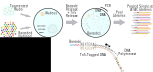
\includegraphics[width=\textwidth]{./ims/dropatac_atac_overview.png}
% \caption[DropATAC Concept]{\textbf{DropATAC Concept.}}
% \label{fig:dropatac_concept}
% \end{figure}

\clearpage
\begin{wrapfigure}{L}{8cm}
\centering
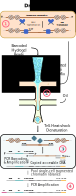
\includegraphics[width=\textwidth/2]{./ims/dropatac_compar_combo.png}
\captionsetup{margin={0pt,0pt},labelfont=bf}
\caption[Drop-ATAC Protocol Overview]{\textbf{Drop-ATAC protocol overview}}
\label{fig:dropatac_compar_combo}
\end{wrapfigure}

1. Isolated nuclei are tagmented in bulk. Tn5 simultaneously cleaves accessible chromatin regions and inserts its adapters at the cleavage site. The Tn5-\acrshort{dna} complex remains intact until denatured.\pms

2. The suspension of "tagmented" nuclei is then run through the same microfluidic device used in our custom inDrop. Here, the single nuclei are now encapsulated together with a barcoded hydrogel bead. The nuclei suspension contains \acrshort{pcr} reagents and \acrshort{dtt}, which mediates release of the barcodes from the hydrogel bead. In the \acrshort{dropatac} protocol, however, the barcode does not contain a poly-T tail to capture poly-A\textsuperscript{+} \acrshort{mrna}, but the sequence complementary to the Nextera Tn5 adapter.\pms

3. The resulting bead-nuclei emulsion then undergoes a heat shock which denatures the Tn5-\acrshort{dna} complex followed by \acrshort{pcr} cycling. During this step, the \acrshort{dropatac} barcodes capture the newly released tagmented \acrshort{dna} fragments and, together with indexed Illumina P5 adapters, act as \acrshort{pcr} primers. In this emulsion \acrshort{pcr}, the tagmented \acrshort{dna} is thus barcoded and i5 indexed.\pms

4. The single-nucleus \acrshort{atac} libraries are now pooled and tagged with Illumina P7 adapters for sequencing in a final adapter \acrshort{pcr}.\pms

\clearpage
\begin{wrapfigure}{L}{9cm}
\centering
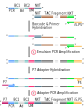
\includegraphics[width=84.452mm]{./ims/dropatac_detail.png}
\captionsetup{margin={6pt,6pt},labelfont=bf}
\caption[Drop-ATAC sequencing library preparation]{\textbf{\acrshort{dropatac} sequencing library preparation.}}
\label{fig:dropatac_detail}
\end{wrapfigure}

What happens during the multiple \acrshort{pcr} steps can be summarised as follows:\pms

1. In the emulsion \acrshort{pcr} step, \acrfull{tac} fragments are captured by barcoded primers released by the hydrogel bead and tagged with an Illumina indexed P5 primer.\pms

2. The barcoded single-cell \acrshort{atac} libraries are pooled and undergo a second \acrshort{pcr} reaction. Here, the barcoded \acrshort{tac} fragments receive a P7 primer, resulting in a sequencing-ready library after subsequent bead purification.\pms

\clearpage
\section{Execution of Drop-ATAC}
\label{sect:dropatac_execution}
Before we arrived at the protocol described in \ref{app:meth_dropatac}, we went through a number of trials in order to find those parameter combinations that would lead to an \acrshort{atac} library ready for sequencing. The reagents used in the preliminary/optimisation stage are described in \ref{app:meth_dropatac_opt}.

\subsection{PCR Emulsion Stability Trials}
% 20190102: stability run: not stable, precipitation in the e2tak mix (dtt and PEG?)
%
\begin{wrapfigure}{R}{\textwidth/3+6pt}
\vspace{-10pt}
\centering
\includegraphics[width=\textwidth/3]{./ims/dropatac_stability1.png}
\captionsetup{margin={0pt,0pt},labelfont=bf}
\caption[Emulsion PCR stability with PEG]{\textbf{Emulsion PCR stability with PEG.}}
\label{fig:dropatac_stability1}
\vspace{-15pt}
\end{wrapfigure}

Previous experiments carried out by a senior lab scientist had already shown that the many successive temperature cycles involved in \acrshort{pcr} destabilise the bead-nucleus emulsion. Since the polymerase mix constitutes a significant part of the droplet volume, we tested whether different polymerase mixes would yield different results in droplet stability. Two \acrshort{pcr} mixes were tested: Takara Bio e2TAK and NEB Q5\textsuperscript{\textregistered}. Both \acrshort{pcr} mixtures were equal in terms of added electrolytes, \acrshortpl{dntp}, and \acrshort{peg} - except for the manufacturer's 5x \acrshort{pcr} buffer supplied with the two polymerases. Droplets were generated according to the general protocol outlined in \ref{app:meth_dropatac}, but without nuclei (dry run). When comparing the droplets pre- and post-\acrshort{pcr}, it became apparent that many of the droplets had merged during thermocycling (figure \ref{fig:dropatac_stability1}), but the emulsion was more stable than previous experiments where all droplets had merged.\pms

% \todo[inline]{Need to check with Suresh - Here, we achieved decent droplet stability. Not perfect, but decent. I believe the difference here is that we used 0.04\% SDS instead of 0.2\% SDS in the lysis mix.}

\begin{wrapfigure}{L}{\textwidth/3+6pt}
\centering
\includegraphics[width=\textwidth/3]{./ims/dropatac_stability2.png}
\captionsetup{margin={0pt,0pt},labelfont=bf}
\caption[Emulsion PCR stability with OptiPrep]{\textbf{Emulsion PCR stability with OptiPrep.}}
\label{fig:dropatac_stability2}
\vspace{-20pt}
\end{wrapfigure}

There was no immediate difference between both \acrshort{pcr} mixes, aside from a marginally better droplet profile in the e2TAK mixture (figure \ref{fig:dropatac_stability2}). However, shortly after preparing the polymerase mixtures, we noticed an occlusion in the e2TAK mix. The precipitate was clearly visible under a microscope and posed danger to the microfluidic operation by clumping nuclei together. We hypothesized that this precipitation could be caused by a reaction between \acrshort{dtt} and \acrshort{peg}, which are both present in the nuclei/\acrshort{pcr} mixture.\pms

%20190103: put the PEG in the enzyme mix, put the BSA in the lysis mix, put optiprep in the pcr mix

Based on these observations, we decided to repeat the trial, but moved \acrshort{peg} from the nuclei-\acrshort{pcr} mix to the \acrshort{bhb} solution. We also added 15\% OptiPrep to the nuclei-\acrshort{pcr} mix (final droplet concentration v/v) in order to reduce nuclei sedimentation and aggregation in the absence of \acrshort{peg}, and 0.1\% \acrshort{bsa} to the lysis mix (final droplet concentration w/v) to further improve droplet stability. The resulting emulsion was very stable, but we still observed precipitation in the nuclei/\acrshort{pcr} mix (figure \ref{fig:dropatac_stability2}). In a final droplet stability and precipitation trial, we omitted all \acrshort{bsa} and \acrshort{peg}, but retained the 15\% OptiPrep and noticed that the precipitation had been heavily reduced. We decided to move forward with the protocol and test the \acrshort{pcr} reaction efficiency.\pms

%20190107 Run 1: Peg/NoPeg and Bulk/Droplet, without EDTA!
\subsection{A Number of Bulk Runs}
\begin{wrapfigure}{R}{\textwidth/2}
\centering
\includegraphics[width=\textwidth/2]{./ims/dropatac_bulkprofile.png}
\captionsetup{margin={6pt,6pt},labelfont=bf}
\caption[Bulk Drop-ATAC Bioanalyzer electropherogram]{\textbf{Bulk Drop-ATAC Bioanalyzer electropherogram.}}
\label{fig:dropatac_bulkdropatac}
\end{wrapfigure}

After the droplet stability and nuclei aggregation issues were reduced (but not completely mitigated), we tested the functionality of the in-droplet \acrshort{pcr} reaction by performing several "bulk" \acrshort{dropatac} runs. In essence, we did not use \acrshortpl{bhb} here, but rather encapsulated the nuclei with the \acrshort{pcr} reagents while the \acrshort{pcr} primers were already dissolved in the nuclei suspension. Such a trial performed by a senior scientist had provided an encouraging Bioanalyzer plot. This run was bare-boned: it omitted most non-necessary additives from the nuclei mix entirely to prevent precipitation or side-effects, using a pre-made NEBNext mix instead. Due to an operation error, the repeated "bulk" run was continued for a moment after the bead and cell suspensions had run out. As the syringes are primed with \acrshort{pbs}, this resulted in the generation of \acrshort{pbs}-filled droplets in the sample emulsion. Despite this error, we decided to process this sample for \acrshort{pcr}, and were pleased to find that the resulting emulsion was very stable post-\acrshort{pcr}, even moreso than the original bare-bones run. A possible explanation for this effect is that the \acrshort{pbs}-filled droplets stabilise the rest of the emulsion. The resulting "bulk" library had a very strong \acrshort{atac}-like electropherogram profile (figure \ref{fig:dropatac_bulkdropatac}). The different peaks and dales show a pitch of around 200 bases, which corresponds to the discrete number of nucleosomes associated with inaccessible \acrshort{dna}. We therefore kept the generation of the \acrshort{pbs} droplets in the following \acrshort{dropatac} runs.\pms

The first "bulk" \acrshort{dropatac} run used NEBNext primers in the emulsion \acrshort{pcr} in order to guarantee that the primer aspect of the reaction was not at fault if the \acrshort{pcr} did not generate \acrshort{dna}. We then performed a second bulk \acrshort{dropatac} run, but replaced the standard NEBNext \acrshort{pcr} primer with our custom barcoded primer. All primers had the same BC1 and BC2 sequence, so there was no variation between the primers used. This run produced \acrshort{dna}, but only about 30\% the amount of the first run (with the NEBNext primer), indicating that the custom \acrshort{pcr} primers do introduce some inefficiency in the reaction. So far, the nuclei remained intact throughout the whole \acrshort{atac-seq} procedure - being present even after \acrshort{pcr} cycling. Before proceeding, we therefore performed another run where the we added Triton X-100 to the bead mix (leading to a final concentration of 1.8\% w/w in the droplets). Such high concentrations of Triton X-100 will lyse the nuclei, and we hoped that this change would lead to an increased yield of \acrshort{dna} post-\acrshort{pcr}. While the nuclei did lyse due to the addition of Triton X-100, there was no \acrshort{dna} post-\acrshort{pcr}. We therefore re-ran with a only 0.36\% Triton X-100 in the droplets, which did produce \SI{80}{\ng} of \acrshort{dna}. This was too low, and combined with a viscous precipitation that appeared only after we started adding Triton X-100 to the mix, we decided to omit Triton X-100 from the final protocol.

% 20190206 Suresh \& Samira: good lead, bulk \acrshort{dropatac} with NEB Next primers, no beads, with bsa, no DTT, no beads, no dna cleaning

% 20190208 Then I replicated that, we got the PBS droplets by accident

% 20190215 Then we did another run with NEBNext poluymeras,e NEBNExt primers, PBS droplets, 1\% bsa, 1\% tween 20, 1\% triton

\subsection{Final Sequencing Library Preparation}
\begin{wrapfigure}{L}{\textwidth/2}
\centering
\includegraphics[width=\textwidth/2]{./ims/dropatac_bioanalyzer.png}
\captionsetup{margin={6pt,6pt},labelfont=bf}
\caption[Electropherogram of final libraries]{\textbf{Electropherogram of final libraries.}}
\label{fig:dropatac_final_electropherogram}
\vspace{-40pt}
\end{wrapfigure}

The final two runs, of which the libraries were both sequenced, had the following properties:\pms

1. In the final "bulk" \acrshort{dropatac} run, a suspension of tagmented MCF7 nuclei was emulsified with a liquid primer mix consisting of the non-uniquely barcoded bead oligo and the indexed P5 primer, as described in figure \ref{fig:dropatac_detail}. We used MCF7 cells as they were readily available to us in the lab. There was no addition of \acrshort{bsa}, \acrshort{peg} or Triton X-100, and we observed no strong precipitation. As described earlier, half the volume of the resulting suspension consisted of \acrshort{pbs} droplets, and the resulting emulsion was very stable post-\acrshort{pcr}.\pms

2. In the true single-cell \acrshort{dropatac} run (\ref{app:meth_dropatac}), tagmented MCF7 nuclei were co-encapsulated with \acrlongpl{bhb}. The beads were washed using the same buffers as used in our custom inDrop protocol. The nuclei suspension now contained \SI{20}{\milli\molar} of \acrshort{dtt} in order to release the barcoded primers from the bead.\pms

After final P7 adapter \acrshort{pcr} and Ampure purification, the \acrshort{pcr} yielded \SI{1075}{\ng} of \acrshort{dna}, but the single-cell \acrshort{dropatac} produced only \SI{193}{\ng} of \acrshort{dna}. This difference in yield can be explained by the reduced \acrshort{pcr} efficiency we observed in previous bulk runs with the custom barcoded primer. The washing buffers used to treat the beads before a high concentration of sodium chloride, which may have affect the \acrshort{pcr} reaction. This washing step, originally tailored for the inDrop protocol, needs to be reviewed and adapted to the \acrshort{dropatac} protocol.\pms

The electropherograms of the two sequencing libraries did not exhibit a strong \acrshort{atac} profile as observed with the earlier "bulk" \acrshort{dropatac} run (figure \ref{fig:dropatac_final_electropherogram}). The single-cell library also showed a strong small fragment peak. This peak was removed in an additional Ampure bead cleaning step.\pms

\section{Sequencing Results}
76\% of the single cell \acrshort{dropatac} and 78\% of the "bulk" \acrshort{dropatac} reads were mapped to the reference genome using \acrshort{star}. Figure \ref{fig:dropatac_igv} shows the coverage of \acrshort{gapdh}. Both datasets showed enriched coverage of the gene's 5' end, indicating an accessible \acrshort{tss}, as expected for a housekeeping genes such as \acrshort{gapdh}. When aggregated, the single cell \acrshort{dropatac} data thus showed good bulk properties.\pms

\begin{figure}[ht]
\centerfloat
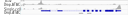
\includegraphics[width=\textwidth]{./ims/dropatac_igv.png}
\caption[Drop-ATAC gene coverage]{\textbf{Drop-ATAC gene coverage.}}
\label{fig:dropatac_igv}
\end{figure}

However, the single-cell \acrshort{dropatac} dataset also had a strong enrichment of 3' fragments which is \textit{the} defining characteristic of our inDrop library. There are a number of ways this can be explained, the most likely one being contamination during library preparation. Since we performed many of the inDrop and \acrshort{dropatac} experiments in parallel, it is possible that a contamination of indexing primers happened during the inDrop library prep. Such a mistake could have led to index collisions, as the inDrop and \acrshort{dropatac} libraries were sequenced on the same flow-cell. We do not believe that the \acrshort{dropatac} library truly contains a large number of 3' fragments, as our protocol cannot capture or amplify them in such large quantities.\pms

Similarly to the inDrop library, we were unable to demultiplex the single-cell \acrshort{dropatac} library due to lack of barcode reads. This problem will further be explored in the next chapter.\pms

% \begin{figure}[ht]
% \centerfloat
% 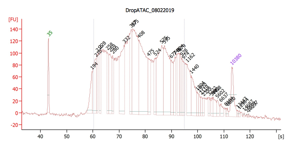
\includegraphics[width=\textwidth]{./ims/dropatac_bulkdropatac.png}
% \label{fig:}
% \end{figure}

% \begin{figure}[ht]
% \centerfloat
% \includegraphics[width=\textwidth]{./ims/dropatac_bioanalyzer.png}
% \caption[inDrop electropherogram]{\textbf{inDrop electropherogram.}}
% \label{fig:}
% \end{figure}
